\documentclass{beamer}

\mode<presentation> {
  \usetheme{CambridgeUS}
  \setbeamercovered{transparent}
}

\usepackage[english]{babel}
\usepackage[utf8]{inputenc}
\usepackage{times}
\usepackage[T1]{fontenc}
\usepackage[backend=biber, style=numeric]{biblatex}
\addbibresource{SeminarTalk.bib}

\title[Wildlife Tracking with IoT]{Using Internet of Things (IoT) Networks for Wildlife Tracking}
\author{Collin Beane}
\institute[U of Minn, Morris]
{
  Division of Science and Mathematics \\
  University of Minnesota, Morris \\
  Morris, Minnesota, USA
}
\date{\today}

\begin{document}

\begin{frame}
  \titlepage
\end{frame}

\begin{frame}
  \frametitle{Outline}
  \tableofcontents
\end{frame}

% Section and subsections will appear in the presentation overview and table of contents.

\section{Background}

\subsection{What is Biologging?}
\begin{frame}{Background}
  \frametitle{Introduction to Biologging}
        \begin{figure}[htbp]
          \centering
          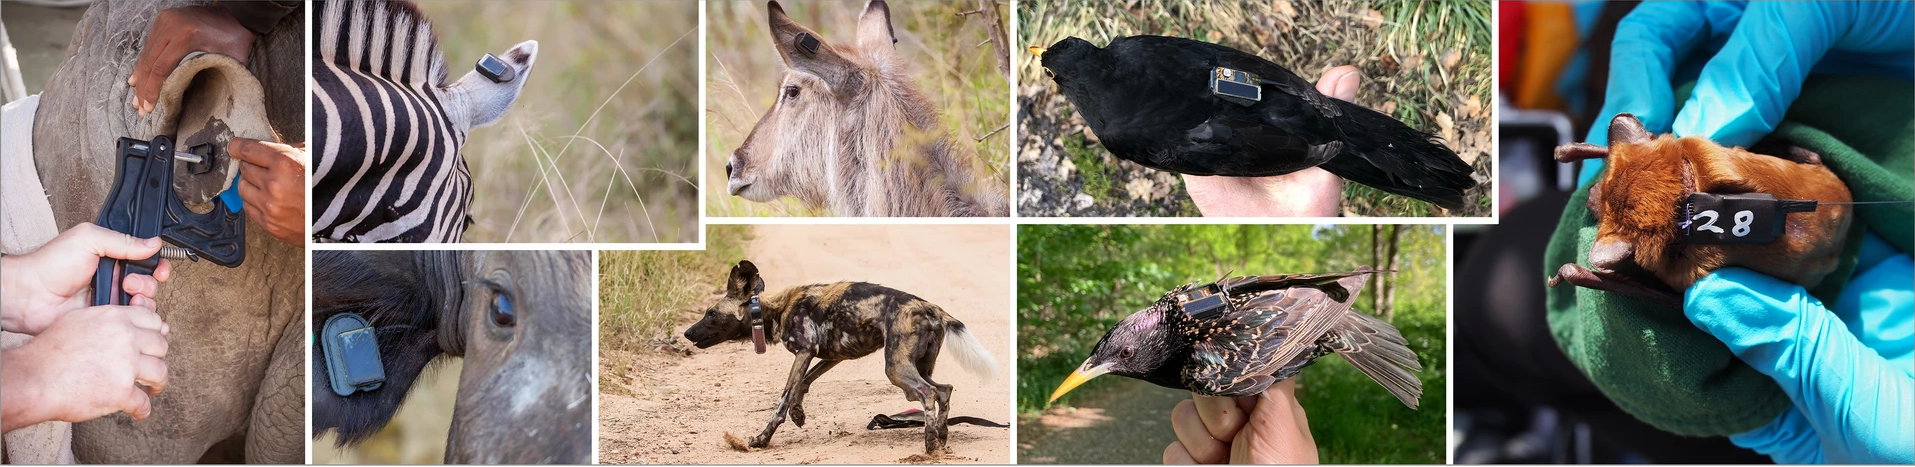
\includegraphics[width=.9\textwidth, height=.25\textheight]{TrakingDevices.png}
          \caption{Animals With SigFox enabled biologging tags\cite{wild2023multi}}
          \label{fig:TaggedAnimals}
        \end{figure}
        \begin{itemize}
          \item Definition: "Investigation of phenomena in or around free-ranging organisms beyond human visibility or experience.\cite{boyd2004bio}"
          \item Method: Tracking wild animals using electronic devices attached to the animal
          \item $\uparrow$ Popularity in early 2000s, practiced since the 60's
          \item Pivotal role in understanding animal behavior and ecology
        \end{itemize}
\end{frame}

\begin{frame}{Background}
  \frametitle{Applications of Biologging}
  \begin{columns}
    \begin{column}{0.5\textwidth}
  \begin{figure}[htbp]
    \centering
    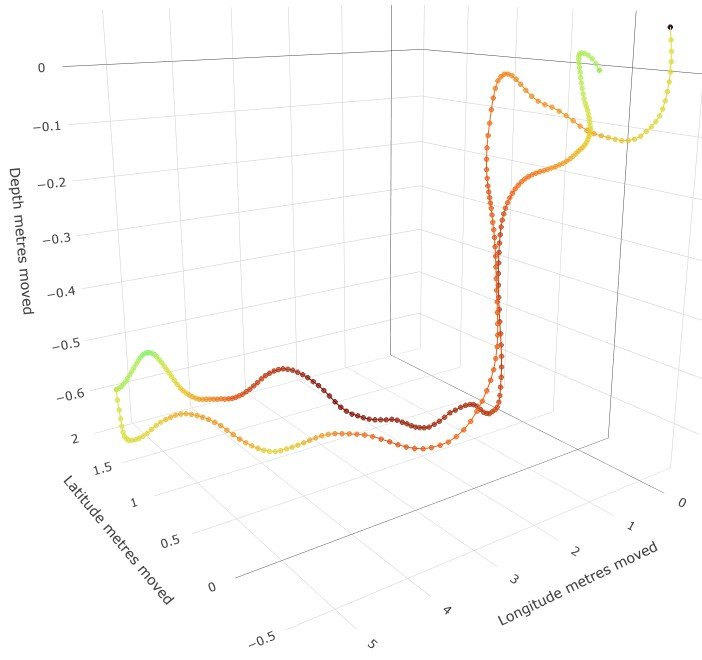
\includegraphics[width=\textwidth]{prairie_dog_map.jpg}
    \caption{3D movement of a prairie dog \cite{Kidangoor_2024}}
    \label{fig:prairie_dog_3D_movement}
  \end{figure}
\end{column}
\begin{column}{0.5\textwidth}
  \begin{itemize}
    \item Track animal movements, behaviors, and migration patterns
    \item Collect data on the animal's environment.
    \item Insights into organisms in hostile or hard-to-reach environments
  \end{itemize}
\end{column}
\end{columns}
\end{frame}

\begin{frame}{Background}
  \frametitle{Impact and Importance}
        \begin{itemize}
          \item Study previously inaccessible aspects of animal life.
          \item Inform conservation efforts and protect endangered species.
          \item Important tool for data collection
          \item Interpretation and application are up to scientists and conservationists.
        \end{itemize}
\end{frame}

\begin{frame}{Background}
  \frametitle{Other Biologging Methods}
  \begin{columns}
    \begin{column}{0.5\textwidth}
        \begin{itemize}
          \item Cellular networks; High Cost
          \begin{itemize}
            \item High Cost/message
          \end{itemize}
          \item Radio Frequency (5-1000m)
          \begin{itemize}
            \item Periodic tracking records
            \item Time stamped data
          \end{itemize}
        \end{itemize}
      \end{column}
      \begin{column}{.5\textwidth}
        \begin{figure}[htbp]
          \centering
          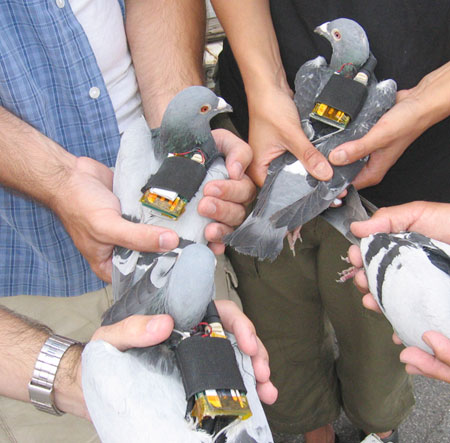
\includegraphics[width=\textwidth]{PigeonCellular.jpg}
          \caption{Pigeons Equipped with cellular trackers \cite{Martin_2006}}
          \label{fig:PigeonCellular}
        \end{figure}
      \end{column}
    \end{columns}
\end{frame}

\subsection{Wireless Networks Basics}

\begin{frame}{Background}
  \frametitle{Data Transmission}
  \begin{columns}
    \begin{column}{0.5\textwidth}
        \begin{figure}[htbp]
          \centering
          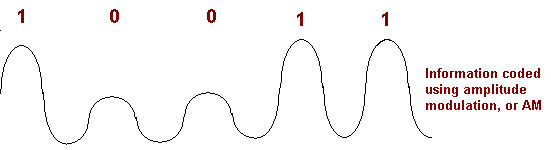
\includegraphics[width=\textwidth]{AMdataTransmission.jpg}
          \caption{How data is represented using amplitude modulation\cite{AMdata}}
          \label{fig:AM_data_transmission}
        \end{figure}
    \end{column}
    \begin{column}{0.5\textwidth}
      \begin{itemize}
        \item Data encoded into 1's and 0's
          \begin{itemize}
            \item Represented by different amplitudes of radio waves
            \item Received and translated by other devices
          \end{itemize}
      \end{itemize}
    \end{column}
  \end{columns}
\end{frame}

\begin{frame}{Background}
  \frametitle{Common Wireless Network Frequencies}
  \begin{columns}
    \begin{column}{0.5\textwidth}
      \begin{itemize}
        \item Home WiFi Frequencies
          \begin{itemize}
            \item 2.4GHz/5GHz/6GHz
          \end{itemize}
        \item LPWAN Frequencies
          \begin{itemize}
            \item $<$1GHz (depends on region)
          \end{itemize}
        \item As frequency increases, range is sacrificed for higher data rates
      \end{itemize}
    \end{column}
    \begin{column}{0.5\textwidth}
      \begin{figure}[htbp]
        \centering
        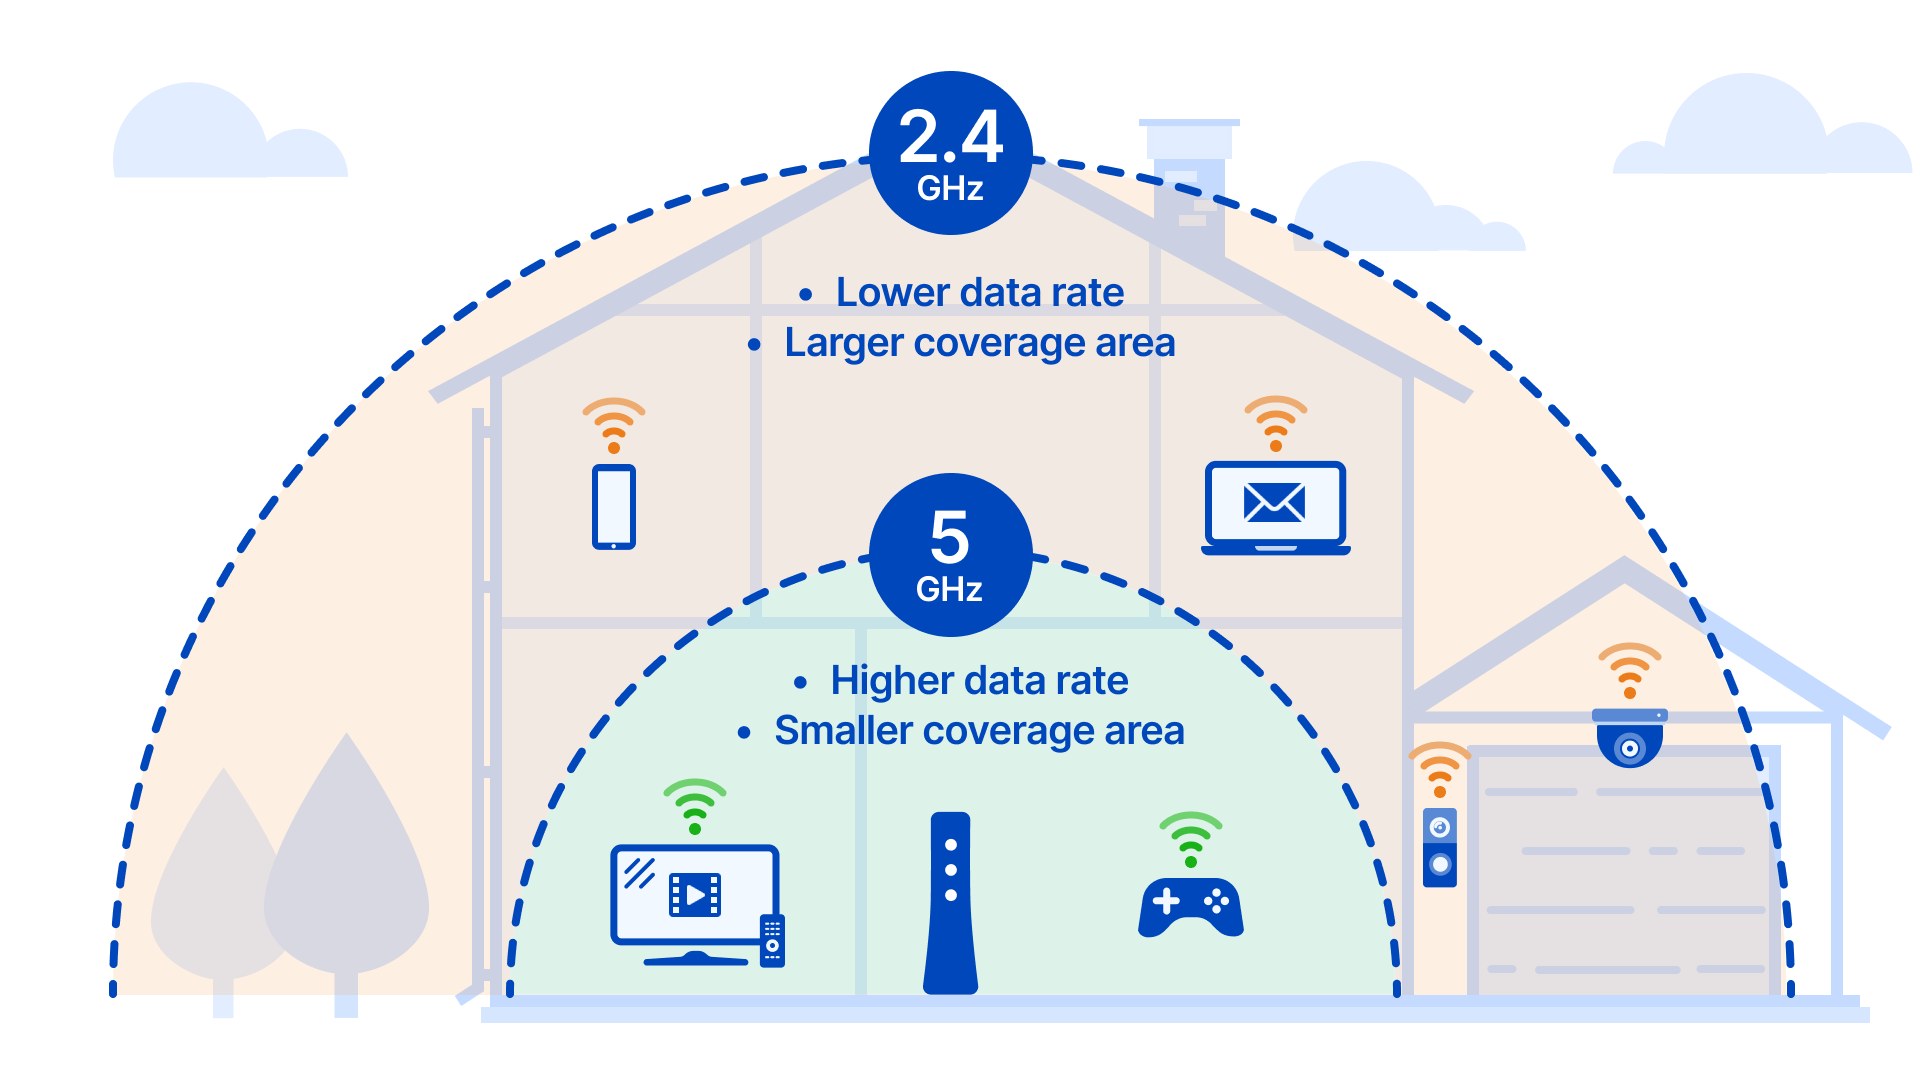
\includegraphics[width=\textwidth]{FreguencyHouse.png}
        \caption{5 GHz will give you more signal strength and faster speed over a shorter range, 
        compared to 2.4 GHz.\cite{CenturyLink}}
        \label{fig:FrequencyHouse}
      \end{figure}
  \end{column}
  \end{columns}
\end{frame}

\begin{frame}{Background}
  \frametitle{Concepts of Wireless Frequencies}
  \begin{columns}
    \begin{column}{0.5\textwidth}
        \begin{figure}[htbp]
          \centering
          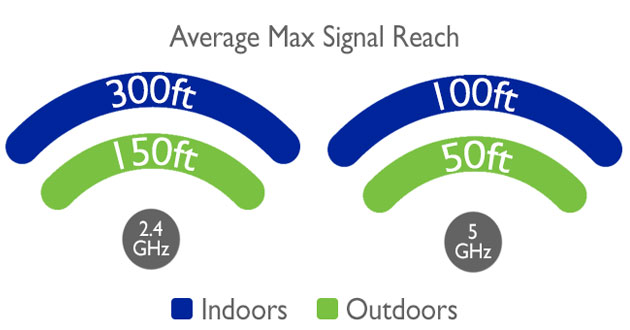
\includegraphics[width=.8\textwidth, height=.20\textheight]{WiFi-frequency-reach.jpg}
          \caption{Comparing Range of frequencies\cite{WiFiFreqImOn}}
          \label{fig:WiFi-frequency-reach}
        \end{figure}
        \begin{figure}[htbp]
          \centering
          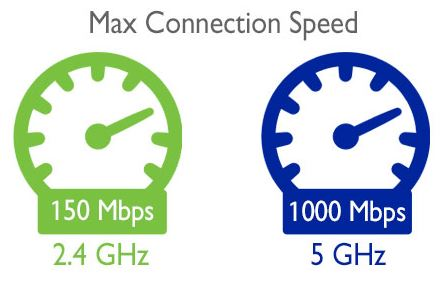
\includegraphics[width=.8\textwidth, height=.20\textheight]{WiFi-frequency-speed.jpg}
          \caption{Comparing Speed of frequencies\cite{WiFiFreqImOn}}
          \label{fig:WiFi-frequency-speed}
        \end{figure}
    \end{column}
    \begin{column}{0.5\textwidth}
          \begin{itemize}
            \item Higher frequency $\Rightarrow$ higher data rates 
              \begin{itemize}
                \item more ones and zeroes received per second
              \end{itemize}
            \item Range is more important than speed in some Applications
            \item Lower frequencies can reach 10's of km vs. 100's of m
          \end{itemize}
    \end{column}
  \end{columns}
\end{frame}

\subsection{What is the Internet of Things?}

\begin{frame}{Background}
  \frametitle{What is the Internet of Things?}
  \begin{itemize}
    \item Empowering physical objects with sensors and software for autonomous interaction
    \item Can either connect via wired or wireless connection
    \item Many applications: Healthcare, agriculture, and of course conservation
  \end{itemize}
\end{frame}

\begin{frame}{Background}
  \frametitle{Layers of an IoT System}
  \begin{columns}
    \begin{column}{0.6\textwidth}
      \begin{itemize}
        \item Application Layer
          \begin{itemize}
            \item Processes and uses data
          \end{itemize}
        \item Network Layer
          \begin{itemize}
            \item Establishes connection to internet and IoT devices
            \item Transmits data to and from the other layers
          \end{itemize}
        \item Perception Layer
          \begin{itemize}
            \item Collects data from the environment or...
            \item Interacts with the physical device
          \end{itemize}
      \end{itemize}
    \end{column}
    \begin{column}{0.4\textwidth}
      \begin{figure}[htbp]
        \centering
        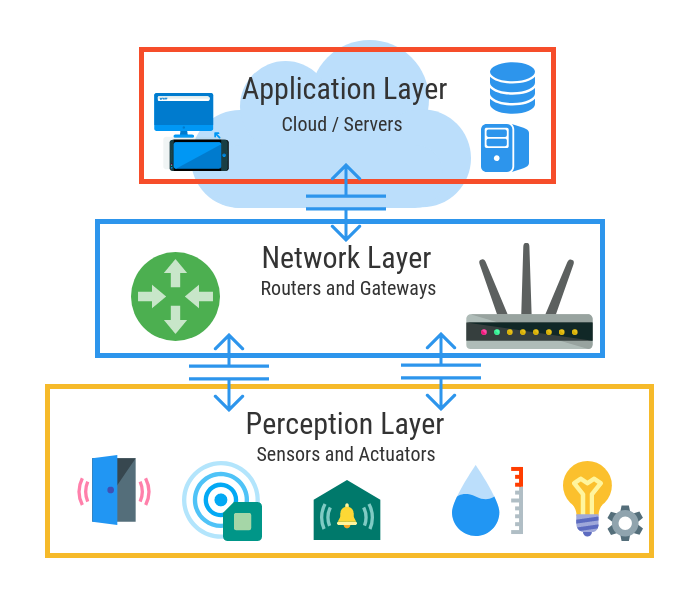
\includegraphics[width=\textwidth]{three-layer-iot-architecture.png}
        \caption{Layer Structure of an IoT System.\cite{Calihman_2021}}
        \label{fig:IoT_Layers}
      \end{figure}
  \end{column}
  \end{columns}
\end{frame}



\section{Components of a Modern Biologging System}
\subsection{Sensor Devices}
\subsection{Base Stations}

\begin{frame}{Components of a Modern Biologging System}
  \frametitle{Sensor Devices}
  \frametitle{Base Stations}
\end{frame}


\section{Networking}
\subsection{LPWAN}
\subsection{LoRaWAN}
\subsection{Traditional Wifi}
\subsection{Comparisons}
\subsection{Security}

\begin{frame}{Networking}
  \frametitle{LPWAN}
  \frametitle{LoRaWAN}
  \frametitle{Traditional Wifi}
  \frametitle{Comparisons}
  \frametitle{Security}
\end{frame}

\section{Challenges to Overcome}
\subsection{Power Consumption}
\subsection{Range}
\subsection{Cost}

\begin{frame}{Challenges to Overcome}
  \frametitle{Power Consumption}
  \frametitle{Range}
  \frametitle{Cost}
\end{frame}

\begin{frame}{References}
  \printbibliography
\end{frame}


\end{document}